\subsection{Outsider detection}
We performed 61*60/2 = 1830 in silico metagenomic experiments involving a total
of 296639 predicted protein-coding sequences, each of which had a hit in at
least 3 other genomes. A total of 67\% of the obtained regression models were
successfully validated and thus allowed the distinction between the sequences
of two genomes. Let us use the Drosophila simulans/Wolbachia in silico
metagenomic experiment as an example of what was done. Figure
~\ref{fig:pca_analysis} shows a principal component analysis (PCA)
visualization of sequence clustering based on the normalized values of
similarity scores for the Drosophila simulans and Wolbachia metagenomic
experiment. A clear separation of sequences can be observed even without the
use of regression analysis by PCA alone; however, we used PCA analysis only for
illustrative purposes.
\begin{center}
\begin{figure}
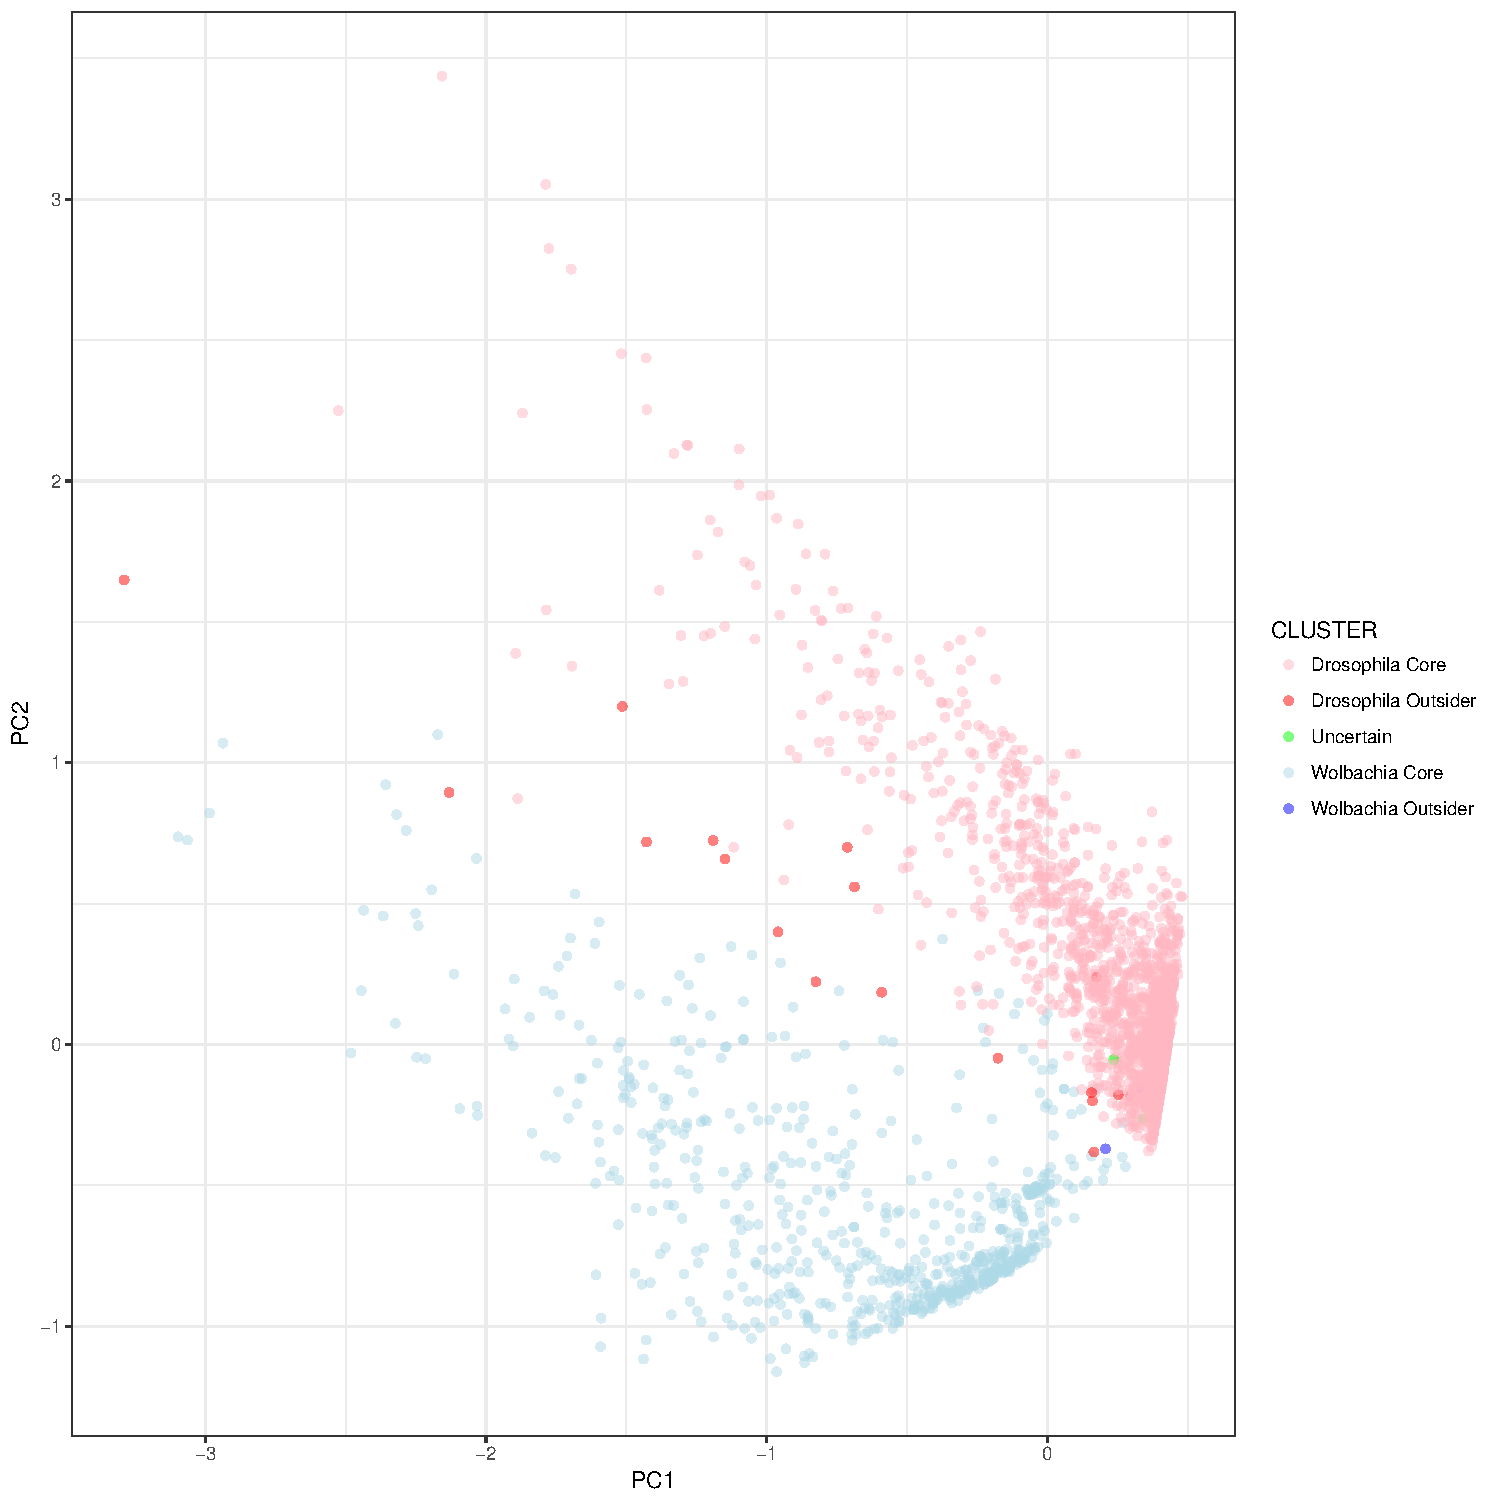
\includegraphics[width=12cm]{w_eds_vs_ds_bootstrapped_pc1_pc2.pdf}
\caption{PCA analysis for clusters of predicted Drosophila simulans
	and Wolbachia genes.}
\label{fig:pca_analysis}
\end{figure}
\end{center}
Figure ~\ref{fig:rsquared_barplot} contains an example result of the regression analysis for Drosophila
simulans and each genome it was compared with. Core genes are sequences from a
genome that were correctly assigned to that genome by the regression analysis.
Outsider genes are sequences that were assigned to another genome.
\begin{center}
\begin{figure}
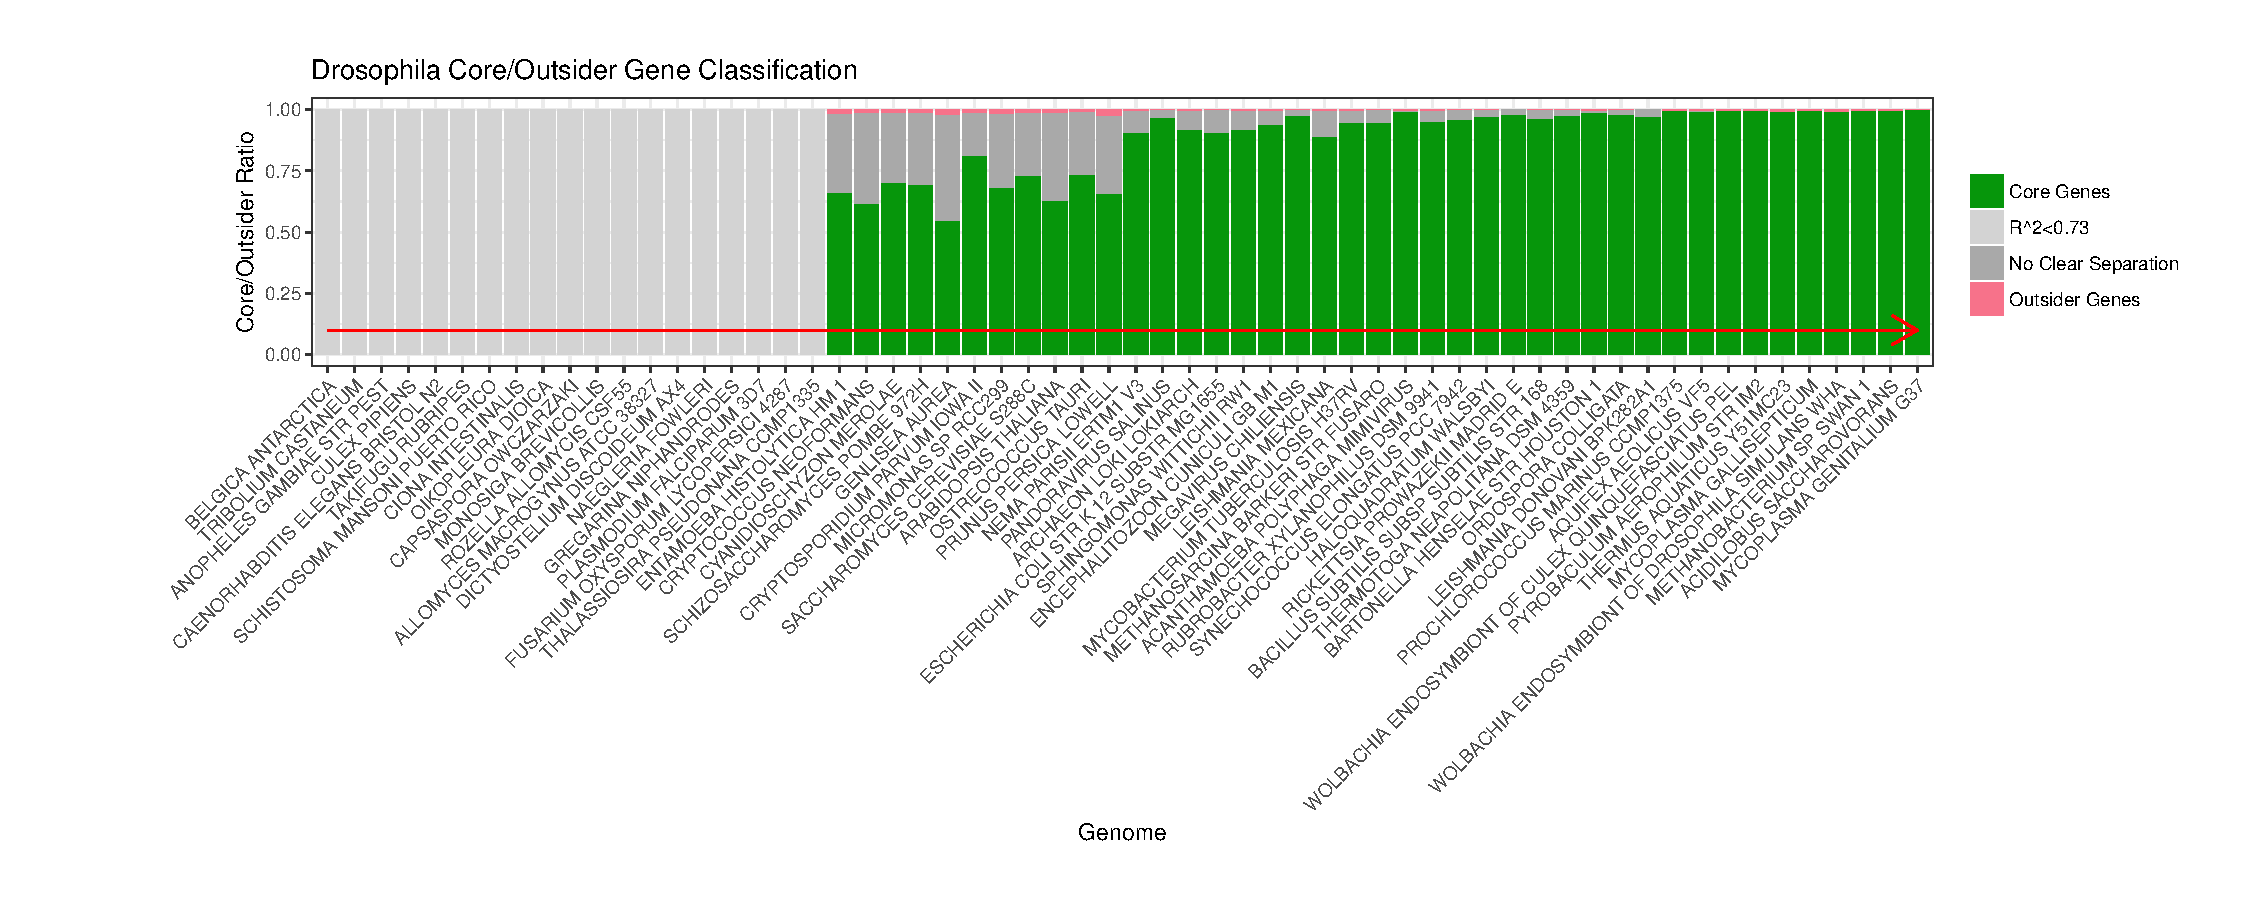
\includegraphics[width=12cm]{core_outsider_barplot_bootstrapped.pdf}
\caption{The fraction of core/outsider Drosophila simulans genes in each in
	silico metagenomic experiment. The gray coloring represents in silico
		metagenomic experiments where separation of genes was not successful (R2 <
				0.73)}
\label{fig:rsquared_barplot}
\end{figure}
\end{center}

Figure ~\ref{fig:rsquared_curve} presents the $R^2$ values obtained in a series of in silico metagenomic
experiments involving Drosophila simulans and each other genome in our dataset
(higher R2 values are better). As expected, we can see that it is nearly
impossible to separate the sequences of Drosophila and closely related
arthropods but it is easy to fulfill this task for distantly related genome
pairs such as Drosophila and Wolbachia.
\begin{center}
\begin{figure}
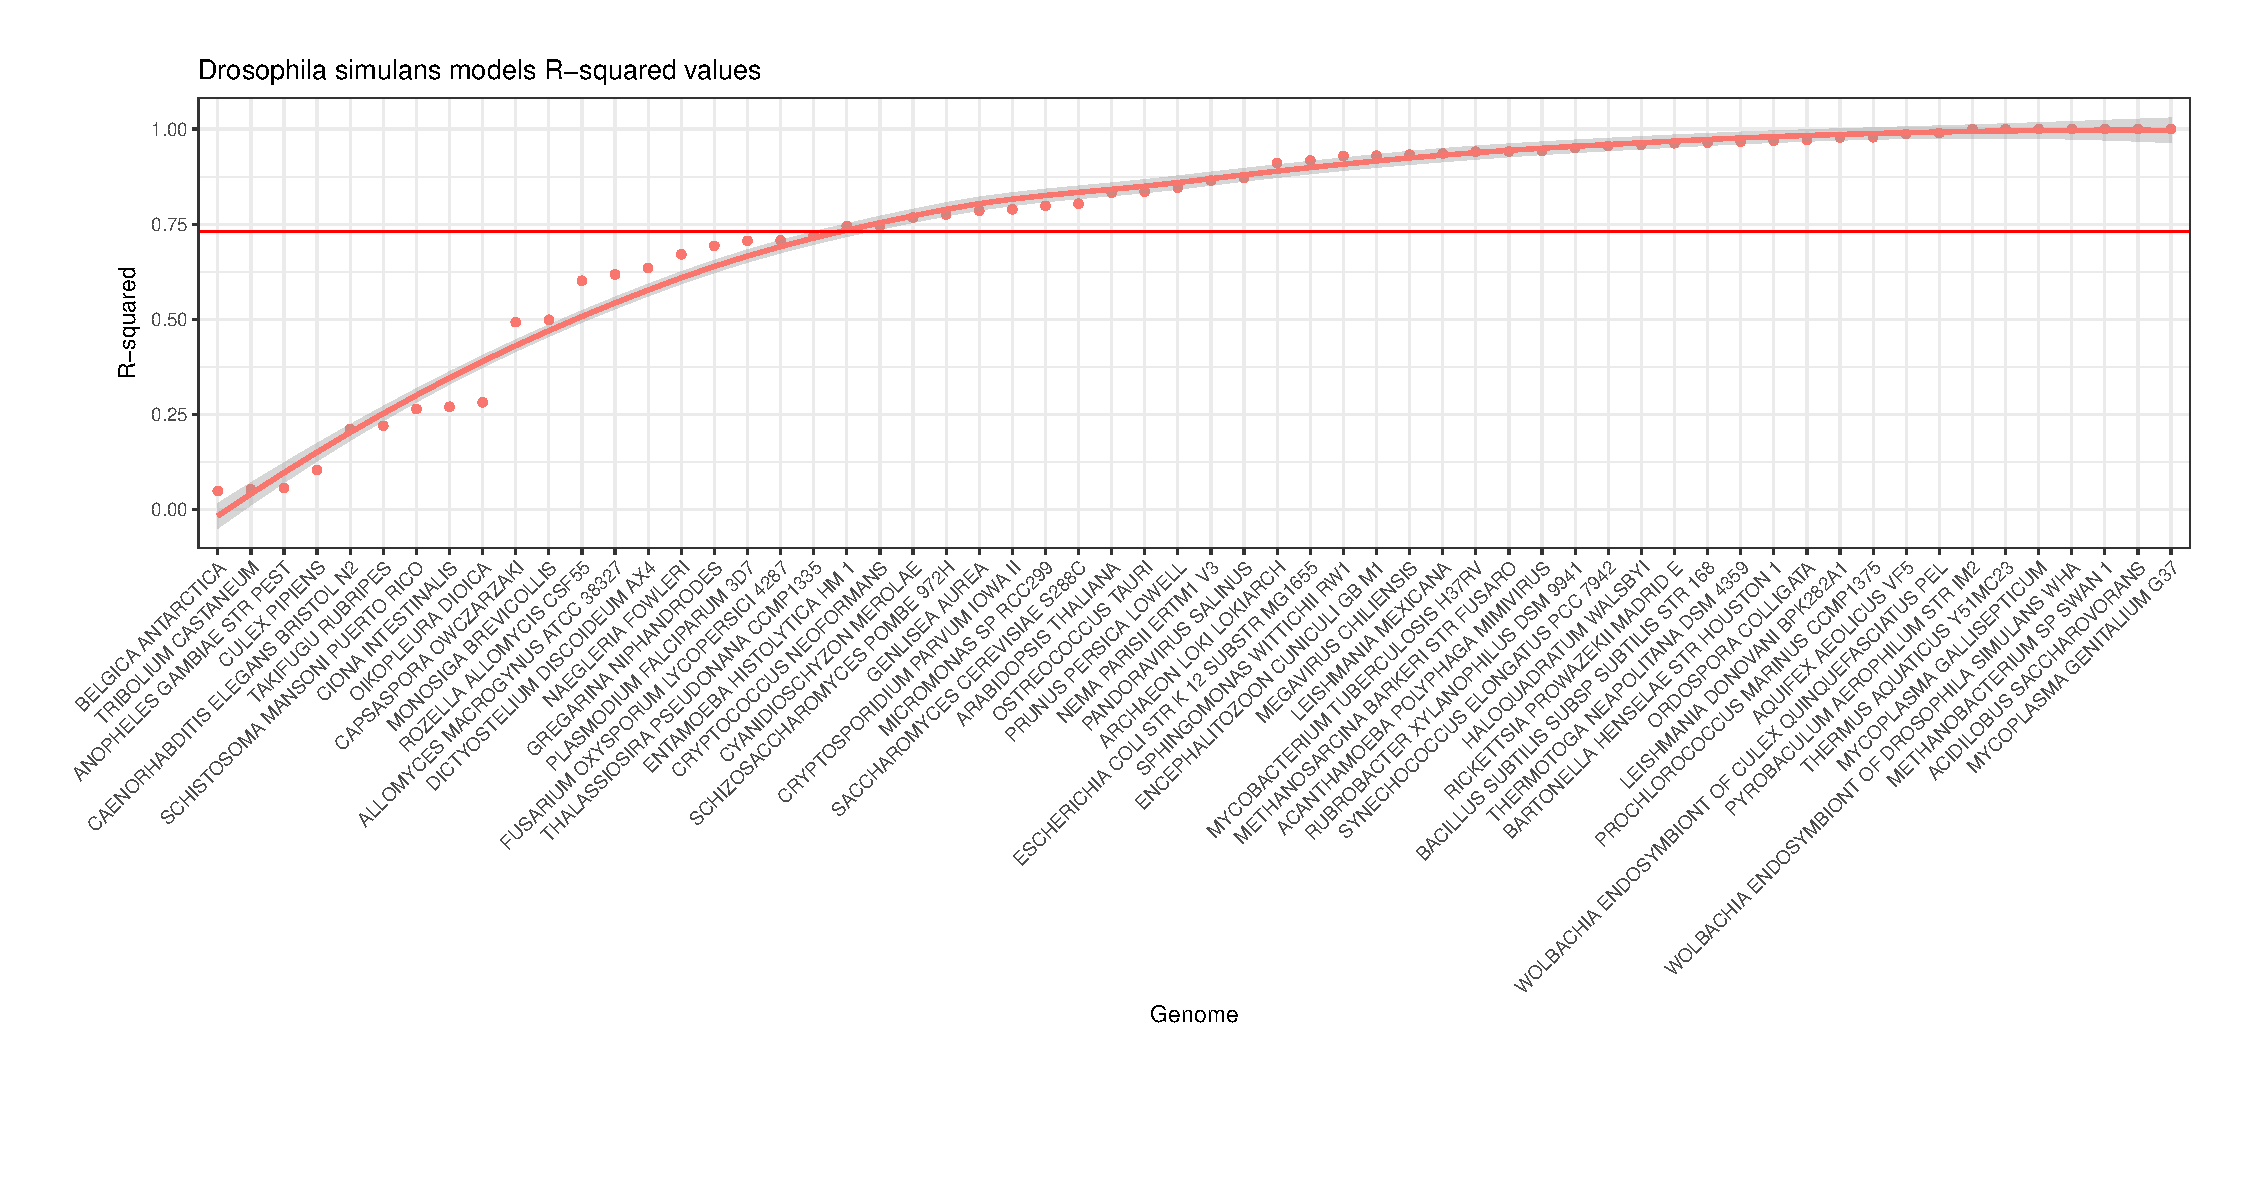
\includegraphics[width=12cm]{rsq_drosoph_bootstrapped.pdf}
\caption{$R^2$ values for in silico metagenomic experiments involving Drosophila simulans genes and genes from one of each other genome}
\label{fig:rsquared_curve}
\end{figure}
\end{center}
The majority of sequences
(288012, 97.1\%) from each analyzed genome were classified as core sequences in
all metagenomic experiment with validated regression models. 4279 (1.4\%) of
the sequences were classified as “outsider once”. The remaining 4348 (1.5\%)
sequences were classified as “outsider multiple” and are the most likely
candidates for HGT. The list of protein-coding open reading frames classified
as “outsider once”, or “outsider multiple” along with their FASTA sequences is
available for download: link. For the fraction of “outsider once” and “outsider
multiple” genes varies from genome to genome see Attachment.
An important limitation is that our approach does not distinguish HGT from genomic
contaminations. Thus the observed differences in Core/Outsider ratio between
different genomes, does not necessarily indicate that some genomes are more
prone to the acquisition of sequences due to HGT. We used a PFAM analysis to
check for any PFAM domains are significantly overrepresented in “outsider
multiple” sets of sequences. A list of top-ranked findings (ranked by
significance) is presented in Table 1.We would like to highlight some of the
most interesting findings.
